\appendix

\section{Supplementary material}

\begin{table}
  \centering
  \begin{adjustbox}{angle=90}
    \begin{tabular}{lrrrrrrrr}
\toprule
{} &  samespeaker &  sameepisode &  sametype &  glovesim &  distance &  durationdiff &  similarity &  similarity\_init \\
\midrule
samespeaker     &         1.00 &         0.21 &      0.01 &      0.02 &     -0.01 &          0.01 &       -0.00 &             0.02 \\
sameepisode     &         0.21 &         1.00 &      0.02 &      0.02 &     -0.01 &          0.00 &        0.02 &             0.03 \\
sametype        &         0.01 &         0.02 &      1.00 &      0.22 &     -0.48 &         -0.03 &        0.03 &             0.02 \\
glovesim        &         0.02 &         0.02 &      0.22 &      1.00 &     -0.10 &         -0.16 &        0.16 &             0.12 \\
distance        &        -0.01 &        -0.01 &     -0.48 &     -0.10 &      1.00 &          0.00 &       -0.00 &            -0.01 \\
durationdiff    &         0.01 &         0.00 &     -0.03 &     -0.16 &      0.00 &          1.00 &       -0.63 &            -0.48 \\
similarity      &        -0.00 &         0.02 &      0.03 &      0.16 &     -0.00 &         -0.63 &        1.00 &             0.81 \\
similarity\_init &         0.02 &         0.03 &      0.02 &      0.12 &     -0.01 &         -0.48 &        0.81 &             1.00 \\
\bottomrule
\end{tabular}

  \end{adjustbox}
  \caption{Variable correlations, dialog pairwise similarity data.}
  \label{tab:dialogvarcor}
\end{table}
\begin{table}
  \centering
  \begin{adjustbox}{angle=90}
    \begin{tabular}{lrrrrrrr}
\toprule
{} &  sameepisode &  sametype &  glovesim &  distance &  durationdiff &  similarity &  similarity\_init \\
\midrule
sameepisode     &         1.00 &      0.01 &      0.01 &     -0.01 &         -0.00 &        0.02 &             0.02 \\
sametype        &         0.01 &      1.00 &      0.40 &     -0.61 &         -0.09 &        0.07 &             0.06 \\
glovesim        &         0.01 &      0.40 &      1.00 &     -0.28 &         -0.22 &        0.26 &             0.18 \\
distance        &        -0.01 &     -0.61 &     -0.28 &      1.00 &          0.07 &       -0.05 &            -0.05 \\
durationdiff    &        -0.00 &     -0.09 &     -0.22 &      0.07 &          1.00 &       -0.51 &            -0.41 \\
similarity      &         0.02 &      0.07 &      0.26 &     -0.05 &         -0.51 &        1.00 &             0.75 \\
similarity\_init &         0.02 &      0.06 &      0.18 &     -0.05 &         -0.41 &        0.75 &             1.00 \\
\bottomrule
\end{tabular}

  \end{adjustbox}
  \caption{Variable correlations, narration pairwise similarity data.}
  \label{tab:narrationvarcor}
\end{table}


\subsection{Targeted Triplets Evaluation Sets}\label{app:targeted_triplets_eval}

To find commonly occurring nouns, adjectives, and verbs, we lemmatize and POS-tag all words in the transcripts of the validation dataset using spacy \citep{honnibal2020spacy}. Afterwards, we identify sets of all nouns $\{n_1, ..., n_n\}$, verbs $\{v_1, ..., v_o\}$ and adjectives $\{a_1, ..., a_p\}$ that occur at least 10 times in the validation data. Given these sets, we create sets of tuples $\{(n_1, n_2), (n_1, n_3), ..., (n_1, n_n), ...,  (n_{n-1}, n_n)\}$ for all combinations of nouns and verbs, respectively. For each of these tuples, we search the validation data for pairs of phrases $(p_k=[w_1, ..., w_x], p_l=[w_1, ..., w_y])$ with same length ($x=y$) and minimal difference regarding the tuple. That is, $n_1 \in p_1$, $n_2 \in p_2$, and if we replace $n_1$ with $n_2$ in $p_1$, it is equal to $p_2$. 

For example, if $n_1 = \text{"peppa"}$ and $n_2 = \text{"george"}$, the phrases $p_1 = [\text{"peppa", "loves", "jumping"}]$ and $p_2 = [\text{"george", "loves", "jumping"}]$ are phrases with minimal differences. A phrase can also be a single word.

We set the minimum phrase duration to 0.3 seconds (for shorter sequences, we do not expect that the video data contains enough semantic information for a model to distinguish between target and distractor). For each phrase $p_1$ we look for the \textit{longest} possible phrase $p_2$. \Cref{fig:num_samples_vs_duration} shows the distribution of samples per duration, \Cref{fig:num_samples_vs_num_tokens} per number of tokens.

Based on each minimal pair, we construct two counter-balanced test triplets as described in the main text.

Figures \ref{fig:num_samples_ADJ_word}, \ref{fig:num_samples_NOUN_word}, and \ref{fig:num_samples_VERB_word} show the number of samples for each adjective, noun and verb.


\begin{figure}
  \centering
  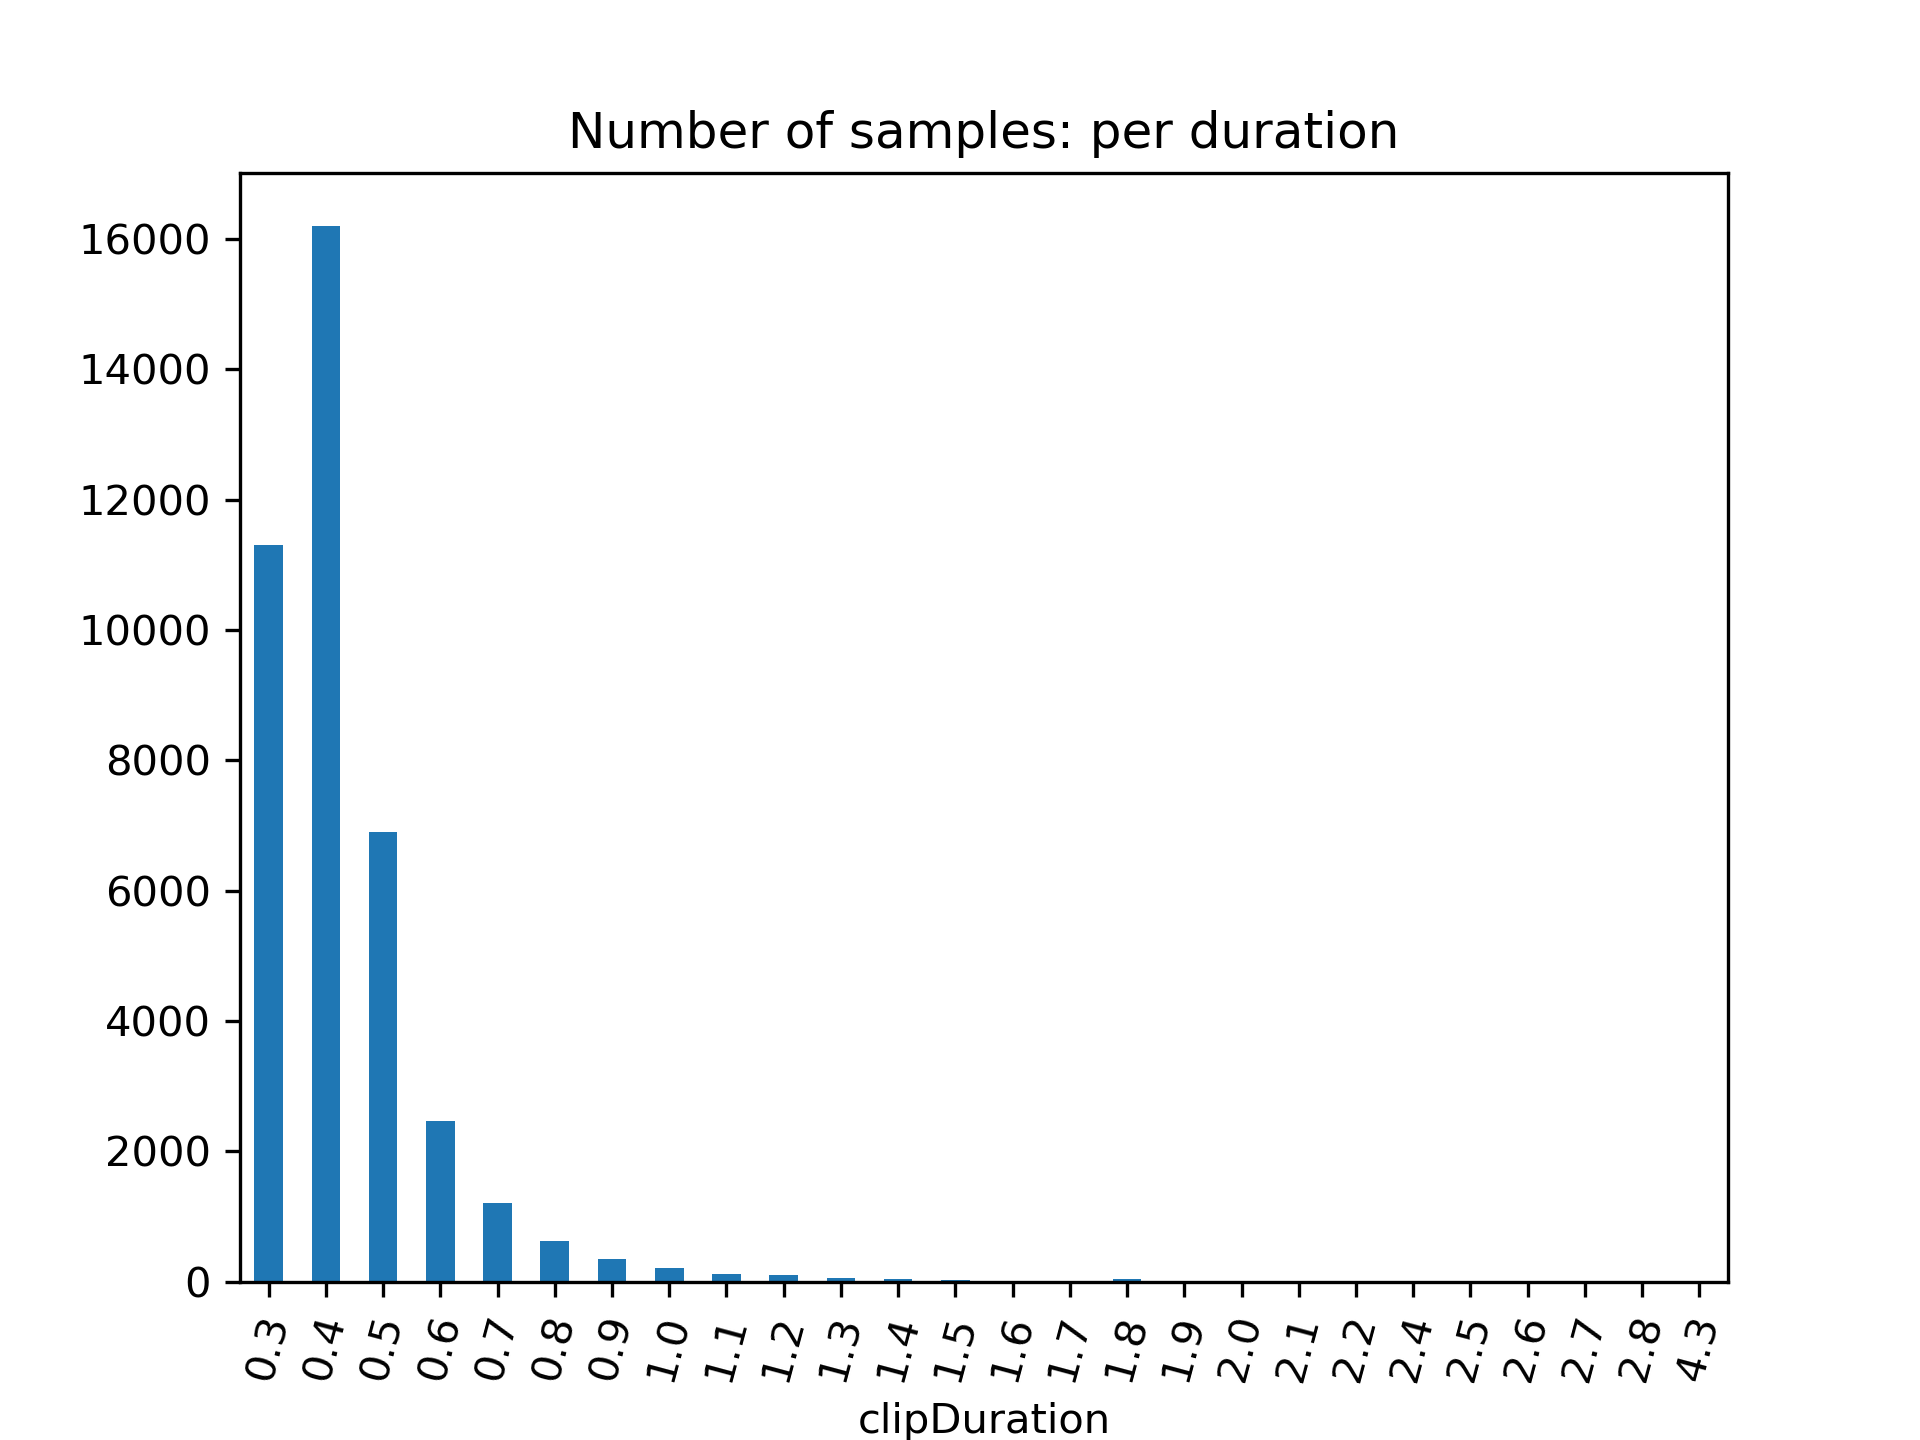
\includegraphics[width=\textwidth]{results/targeted_triplets/num_samples_vs_duration.png}
  \caption{Number of samples per duration}
  \label{fig:num_samples_vs_duration}
\end{figure}


\begin{figure}
  \centering
  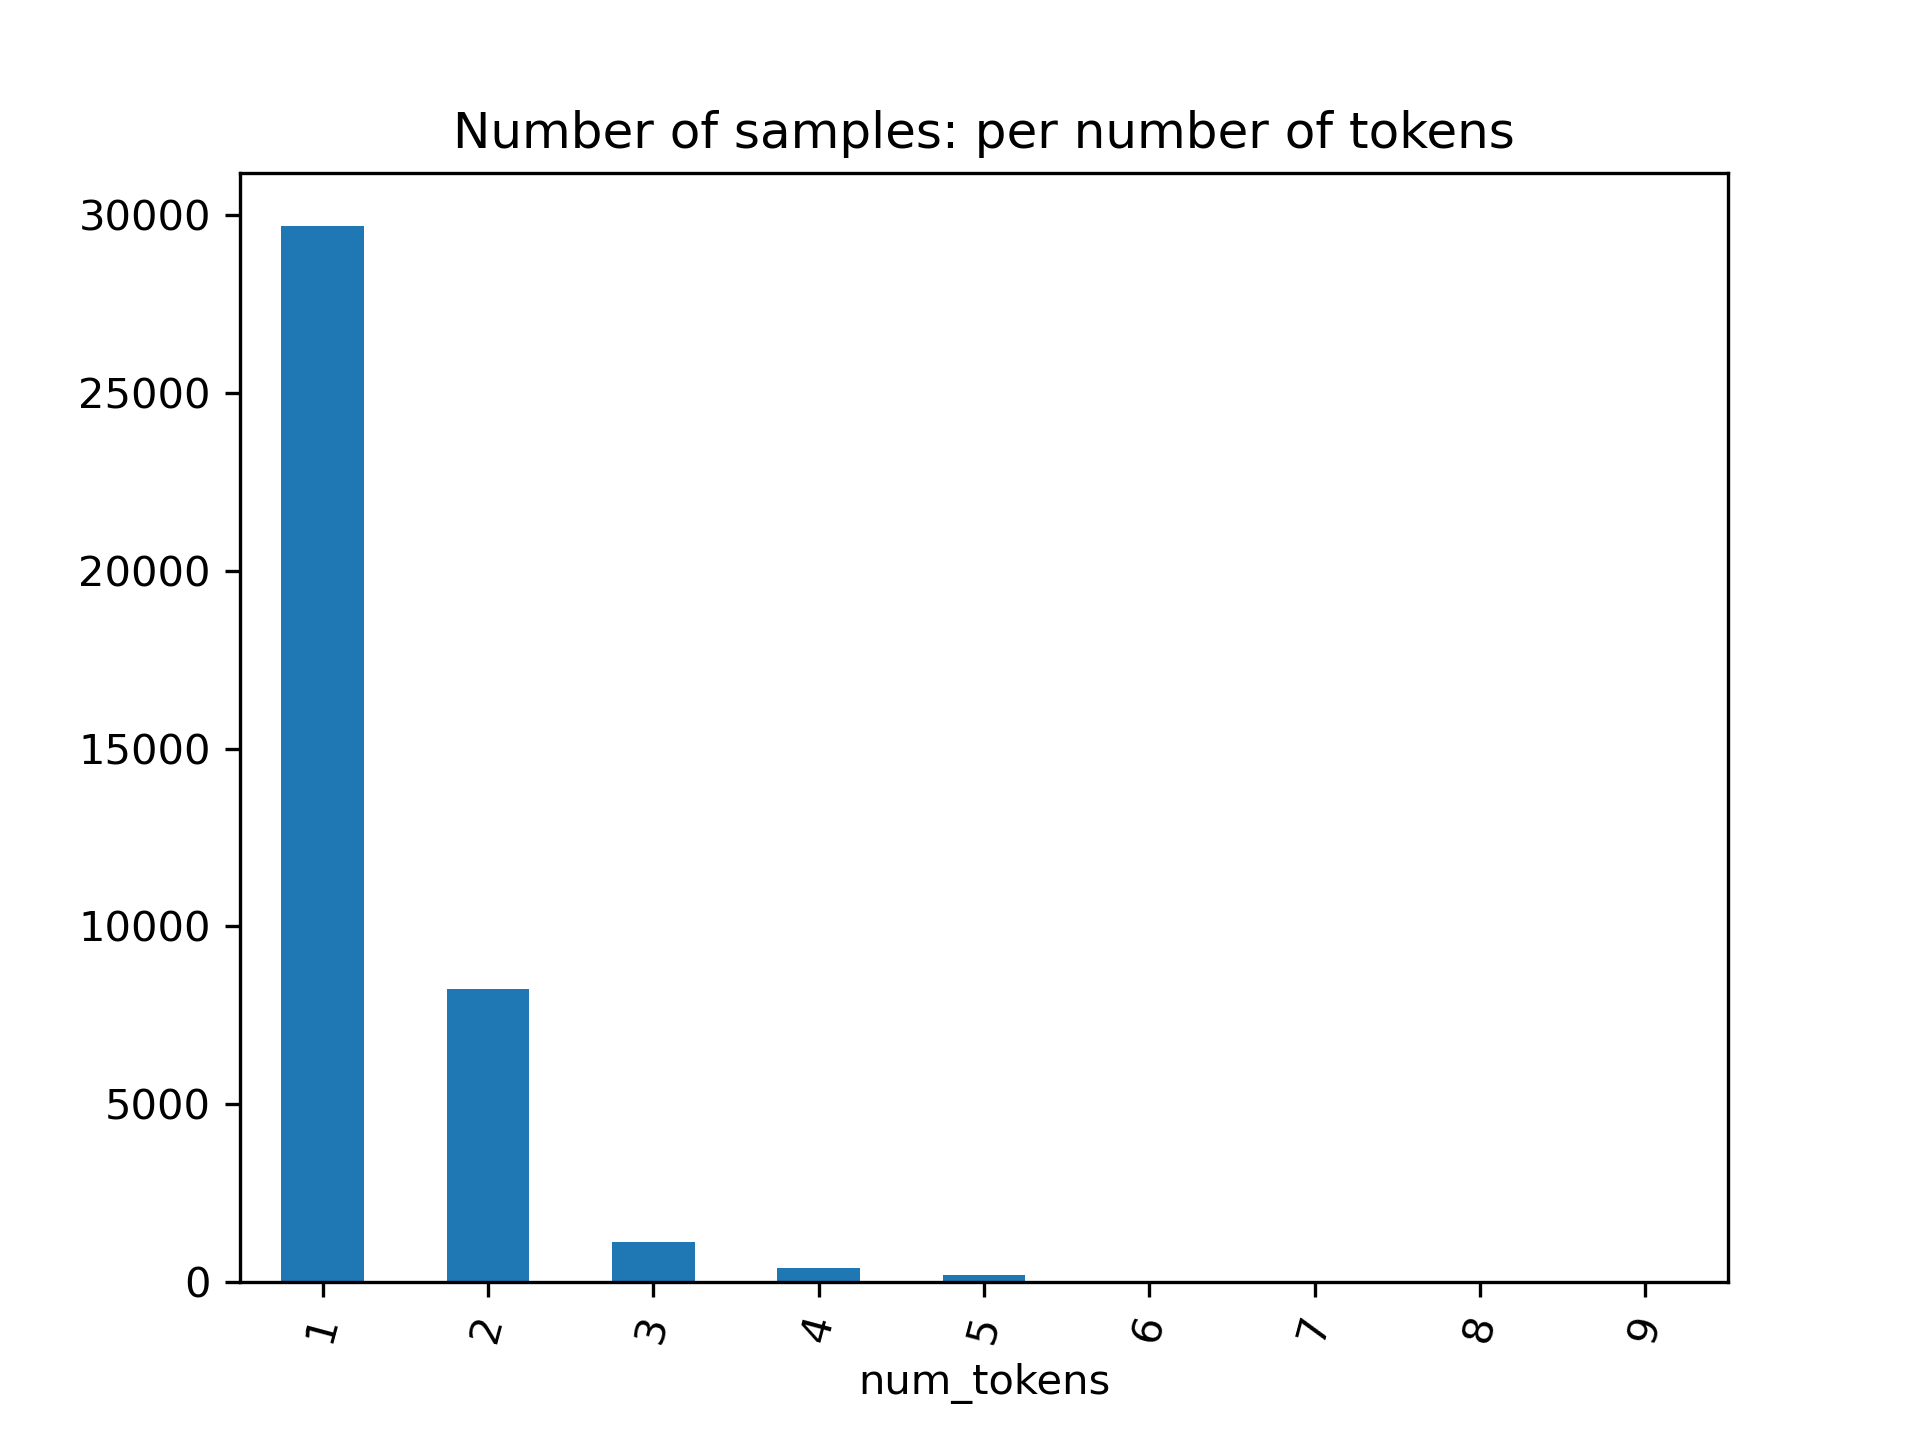
\includegraphics[width=\textwidth]{results/targeted_triplets/num_samples_vs_num_tokens.png}
  \caption{Number of samples per number of tokens}
  \label{fig:num_samples_vs_num_tokens}
\end{figure}


\begin{figure}
  \centering
  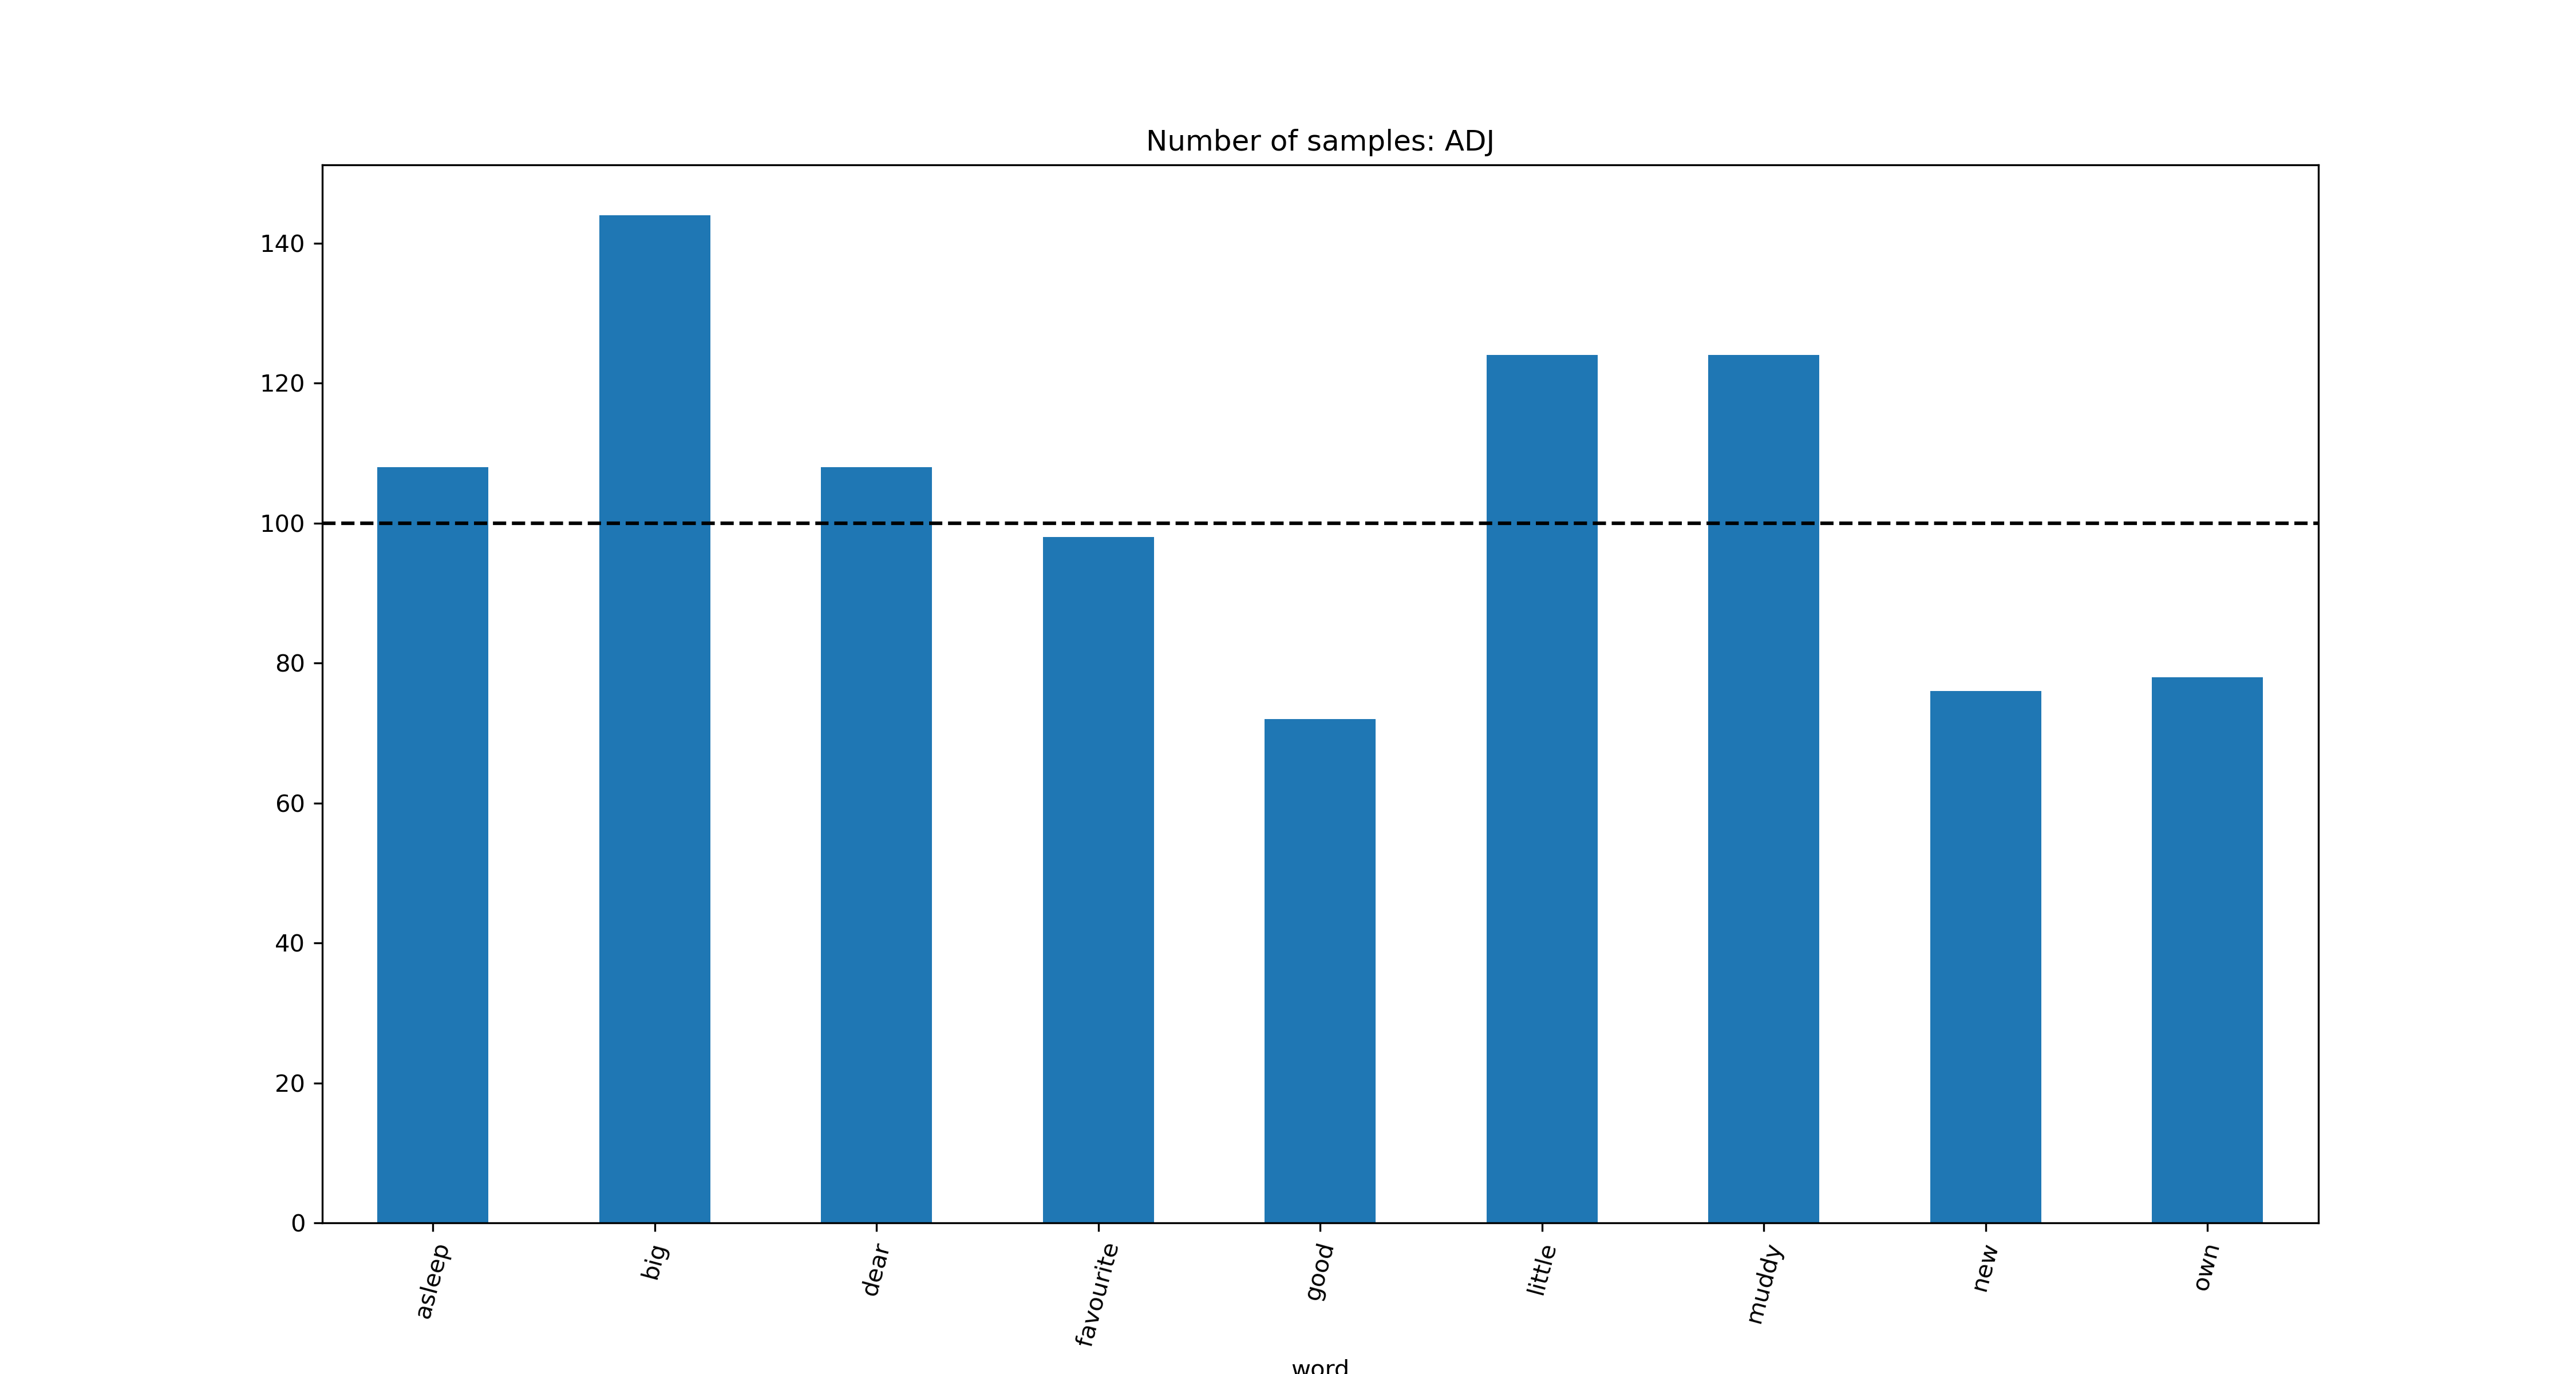
\includegraphics[width=\textwidth]{results/targeted_triplets/num_samples_ADJ_word.png}
  \caption{Number of samples: adjectives}
  \label{fig:num_samples_ADJ_word}
\end{figure}

\begin{figure}
  \centering
  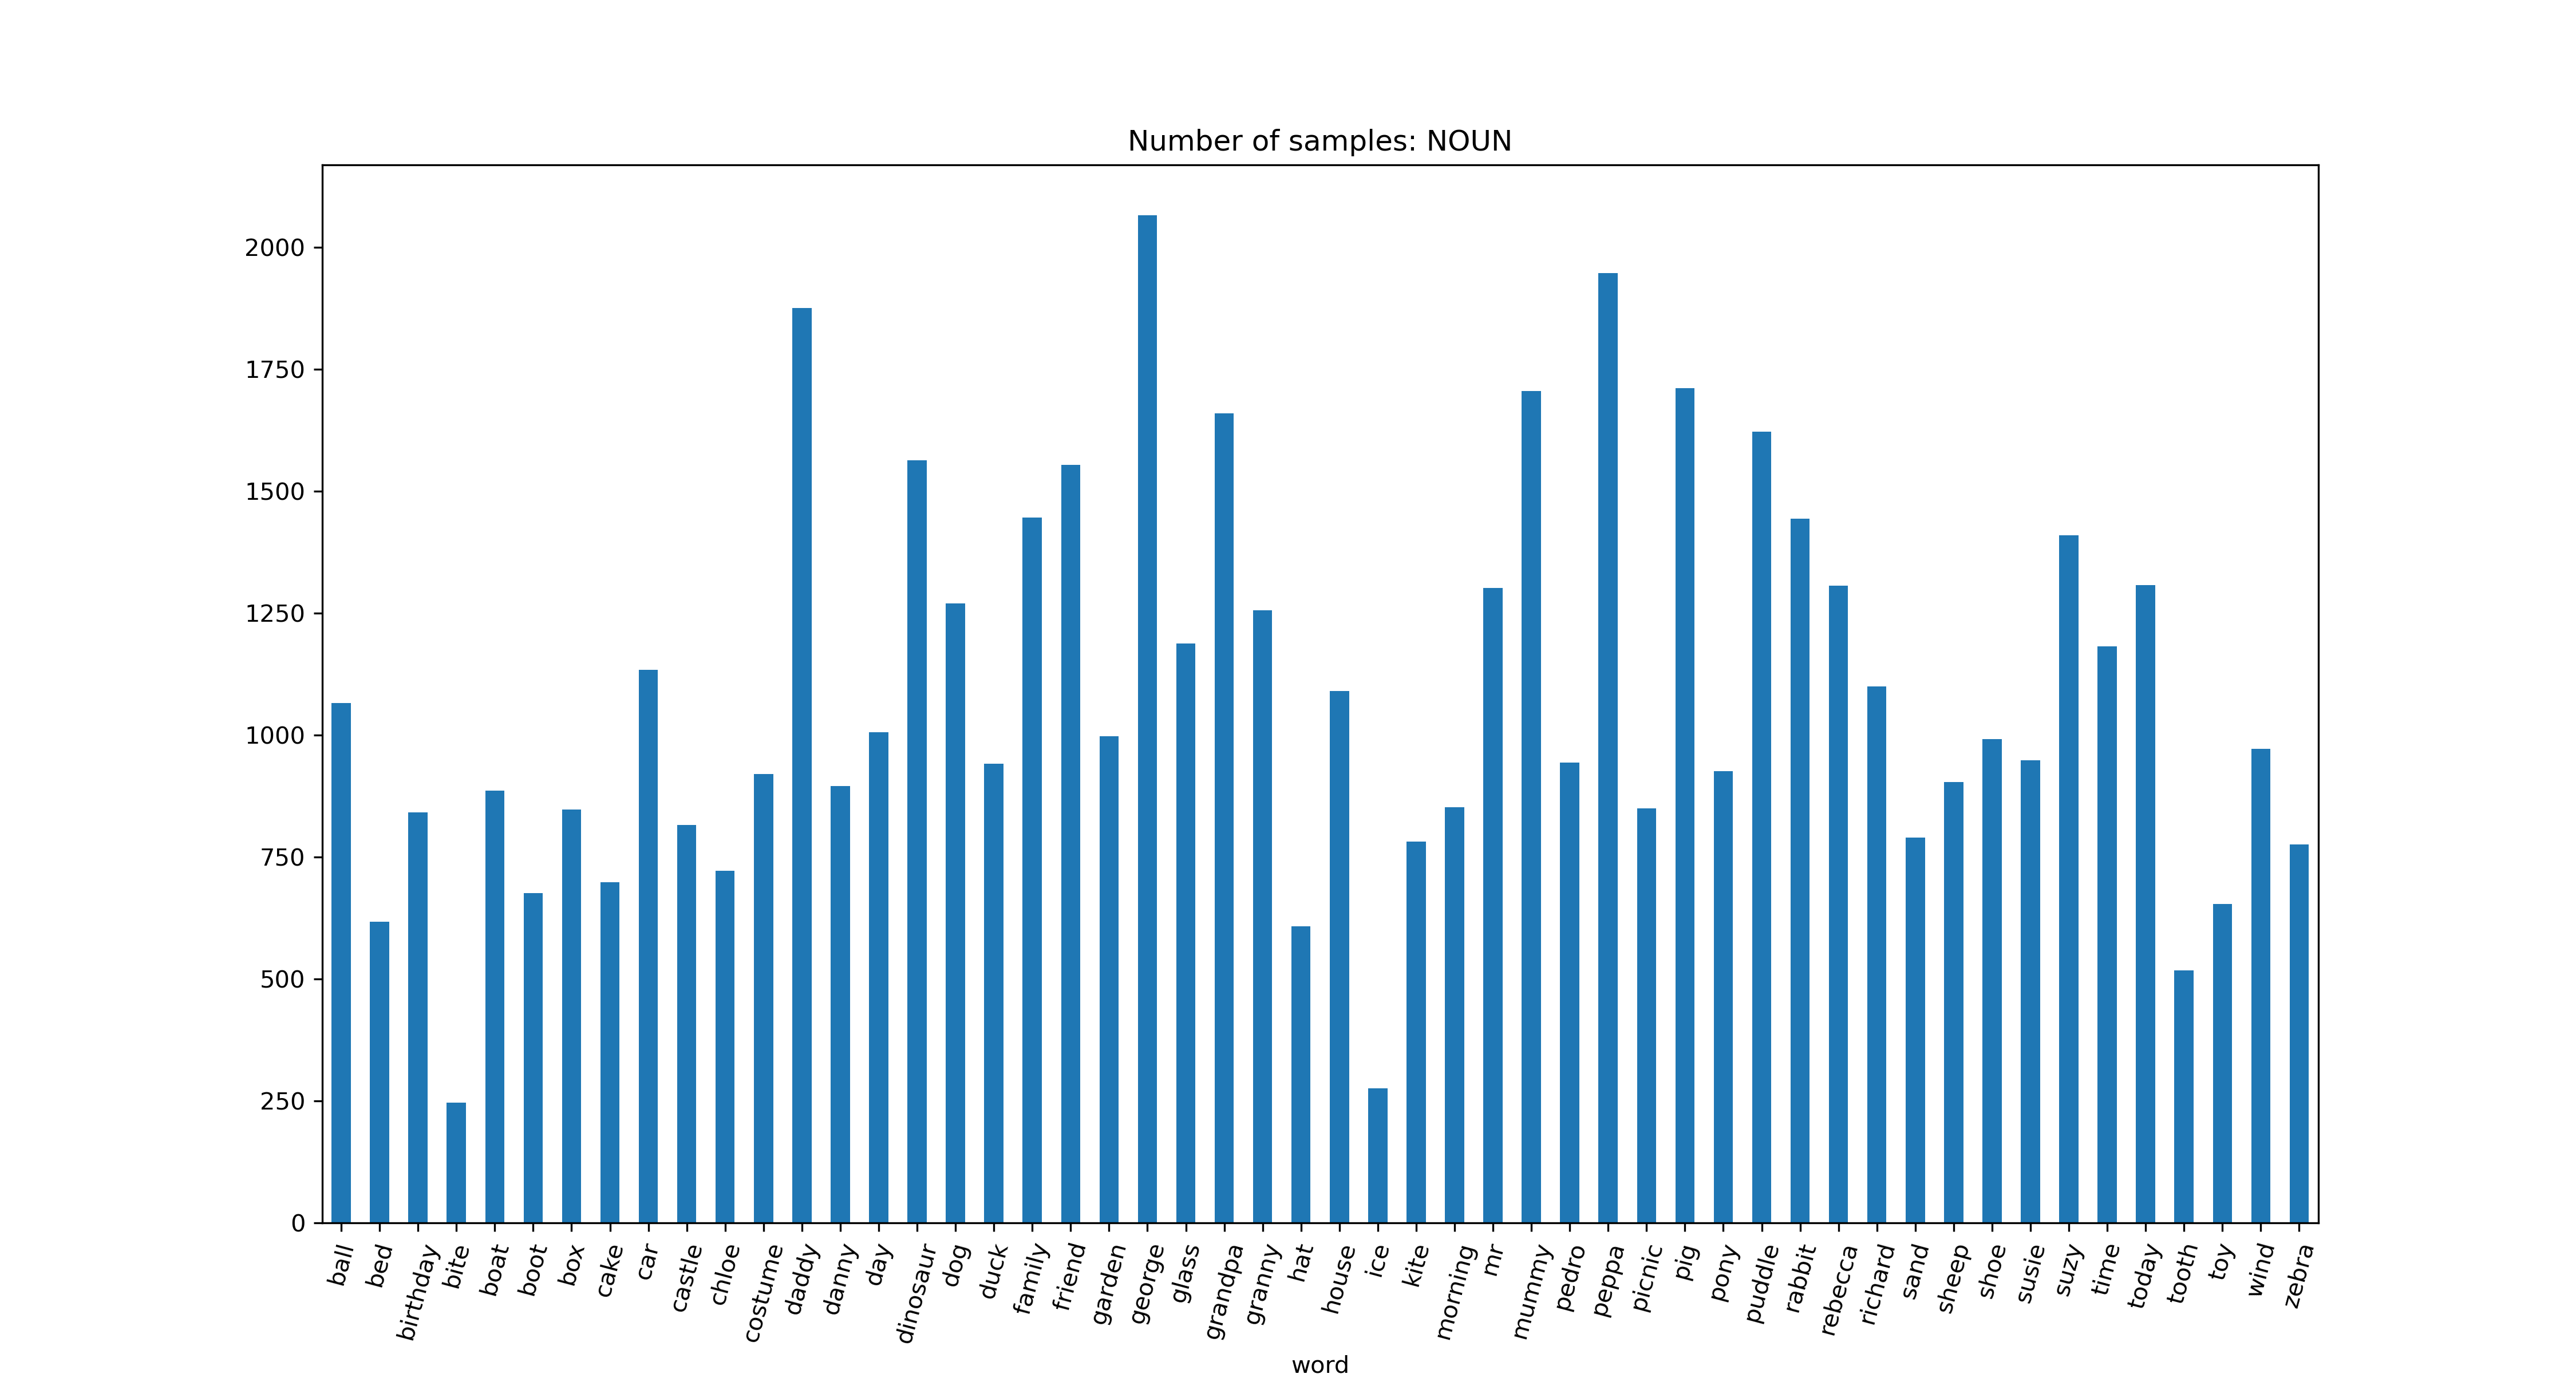
\includegraphics[width=\textwidth]{results/targeted_triplets/num_samples_NOUN_word.png}
  \caption{Number of samples: nouns}
  \label{fig:num_samples_NOUN_word}
\end{figure}

\begin{figure}
  \centering
  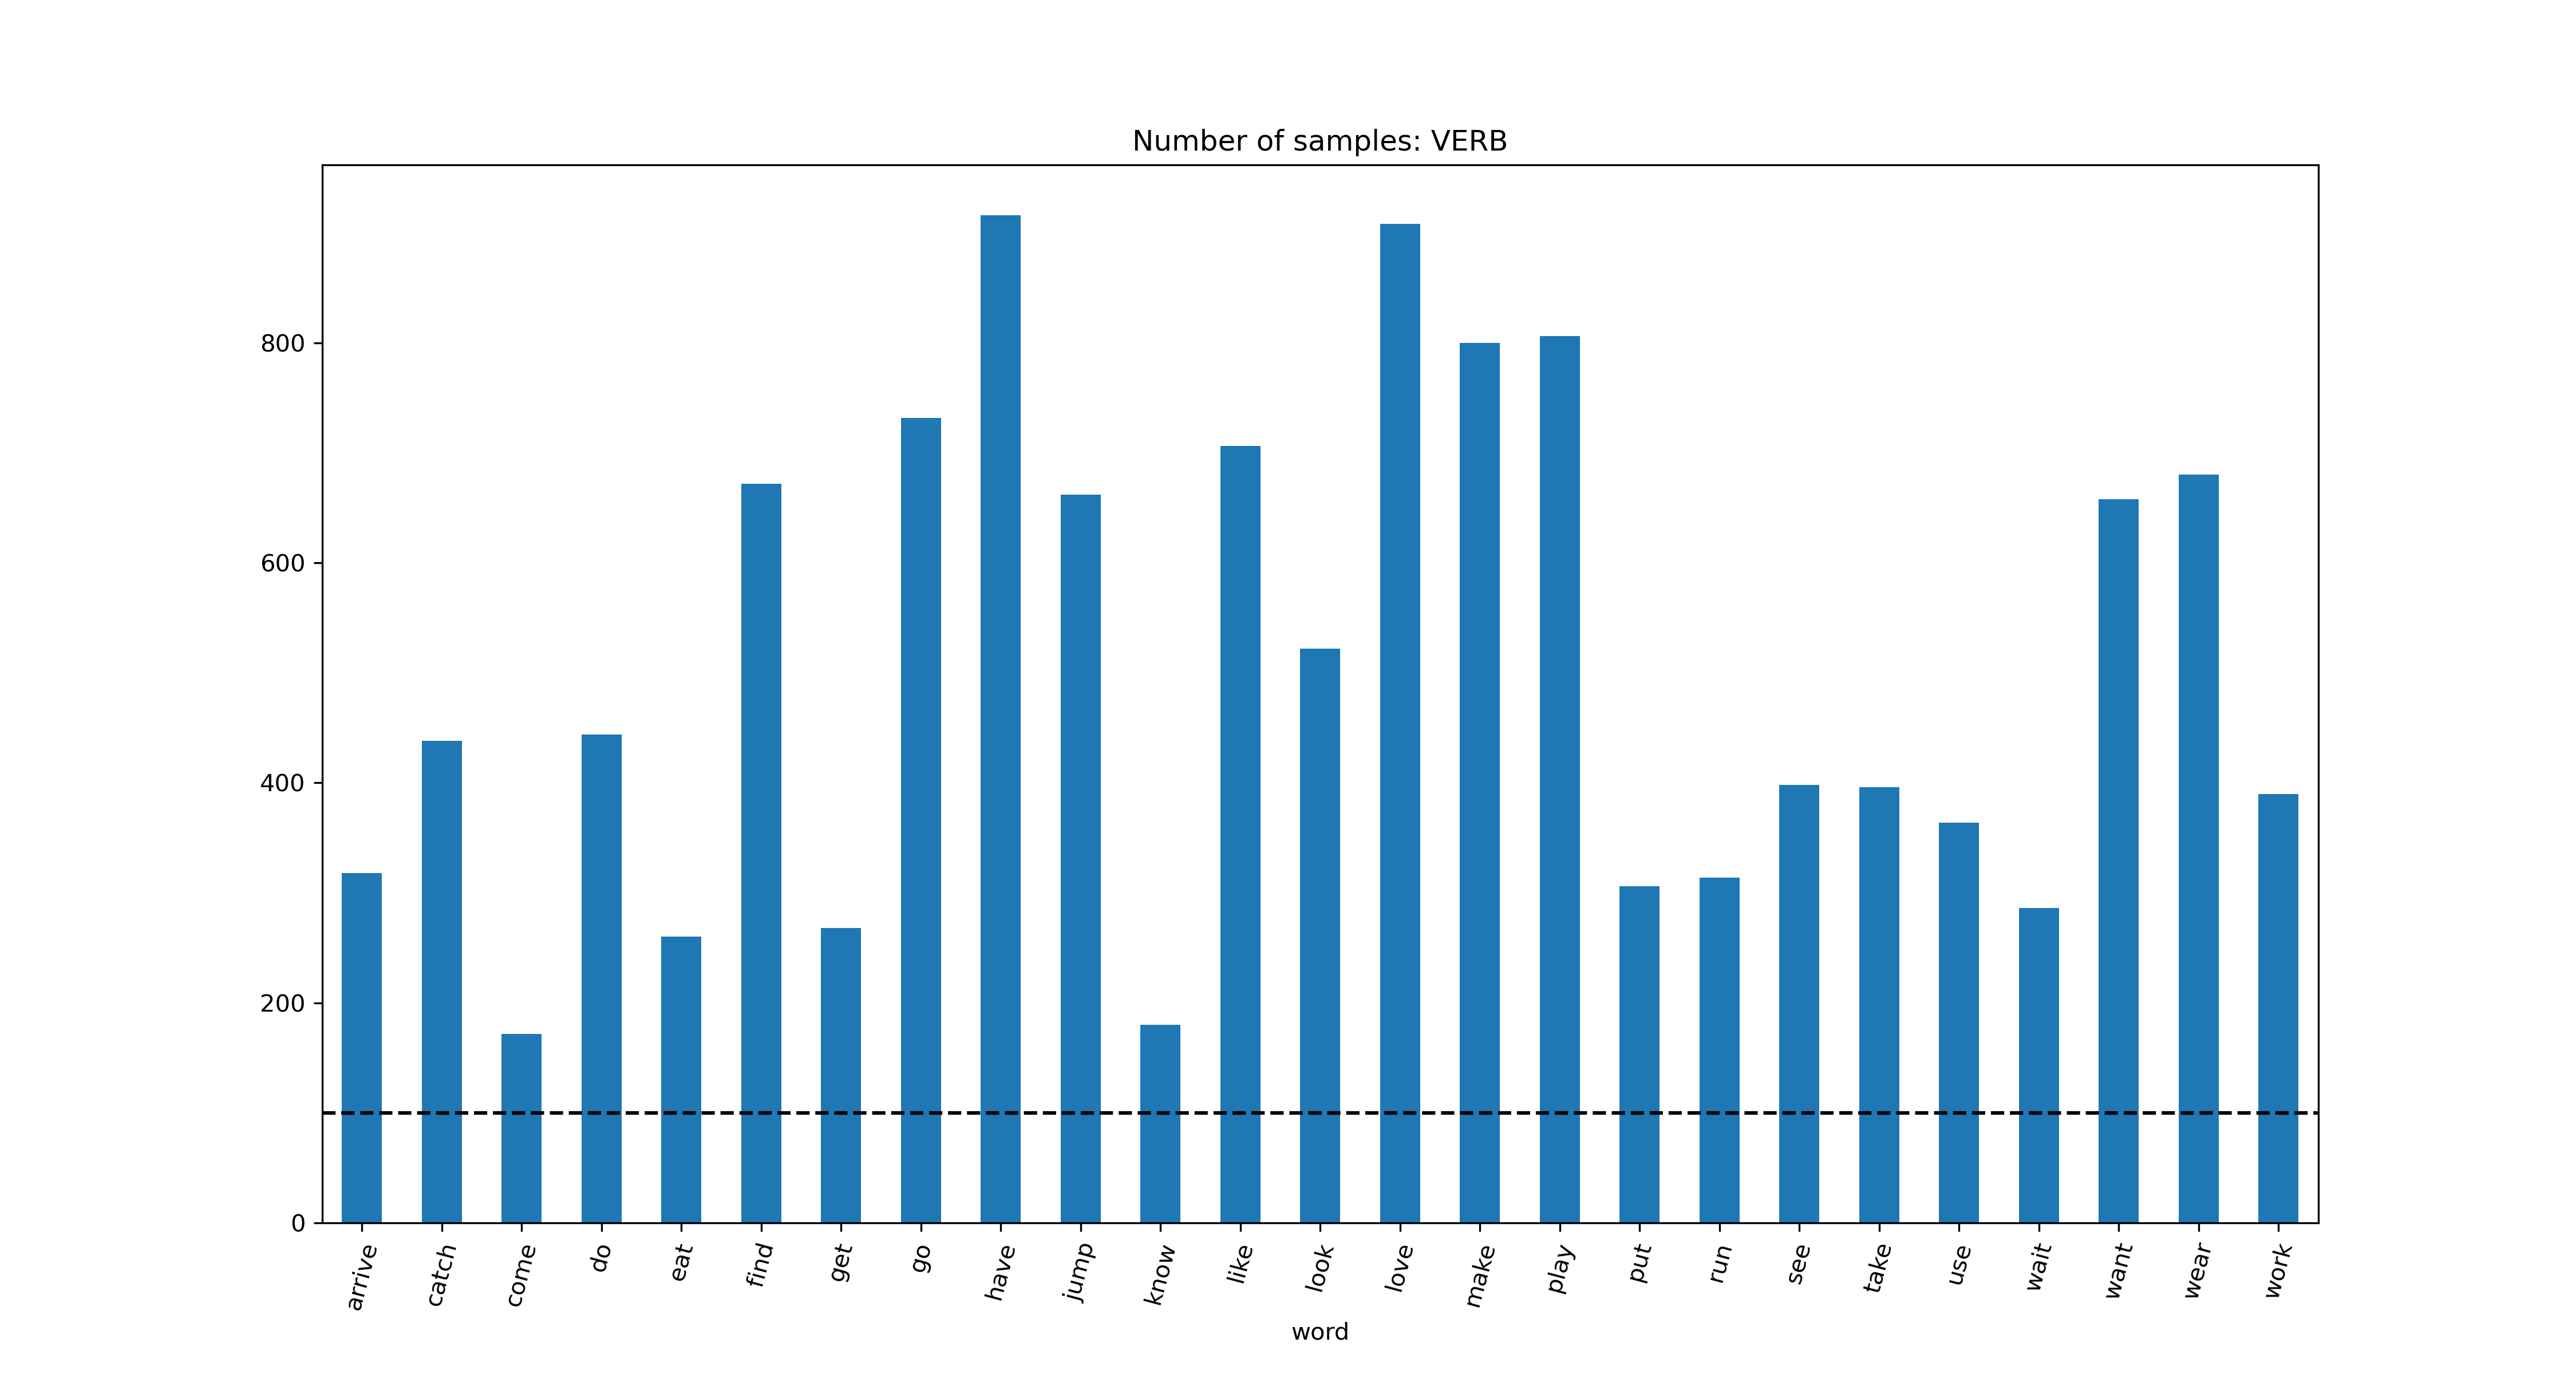
\includegraphics[width=\textwidth]{results/targeted_triplets/num_samples_VERB_word.png}
  \caption{Number of samples: verbs}
  \label{fig:num_samples_VERB_word}
\end{figure}

